\documentclass[12pt]{article}
\usepackage{packages}
\usepackage[compat=1.1.0]{tikz-feynman}

% !TeX program = lualatex

\begin{document}

\centerline{\Large\bfseries Building supersymmetric models using superfields}
\vspace{5pt}
\centerline{\large Seminar on Supersimmetry}

\vspace{50pt}

\begin{figure}[h]
  \centering 
  
\includegraphics[scale=0.45]{images/uniheilogo.png}
\end{figure}

\vspace{50pt}

\centerline{University of Heidelberg, Summer Semester 2022}
\vspace{5pt}
\centerline{Matteo Zortea}
\vspace{5pt}
\centerline{Coordinated by prof. Joerg Jaeckel}

\newpage
Part on $\mathcal{L} \to \mathcal{L} + \partial_\mu f$ \\
\raggedright The two main ingredients of a supersymmetric theory in the superspace formalism, are the chiral and vector superfields. Let us briefly recall some of their properties, useful for the subsequent reasonings. \\
\vspace{15pt}
A left-chiral superfield $\Phi$ (right-chiral superfield $\chi$) is obtained by imposing the constrain $\bar D_{\dot \alpha} \Phi(x, \theta, \bar\theta) = 0$  ($D_{\alpha} \chi(x, \theta, \bar\theta) = 0$), and a general expansion in powers of $\theta, \bar\theta$ reads
\begin{equation}
\begin{gathered}
  \Phi(x, \theta, \bar\theta) = \varphi(x) + i\bar\theta \bar\sigma^{\mu}\theta \partial_{\mu}\varphi(x) + \frac{1}{4}\theta\theta\bar\theta\bar\theta\partial_{\mu}\partial^{\mu}\varphi(x) + \sqrt{2}\theta\psi(x) + \\ 
                -\frac{i}{\sqrt{2}}\theta\theta\bar\theta\bar\sigma^{\mu}\partial_{\mu}\psi(x) + \theta\theta F(x)
\end{gathered}
\label{eq:leftchiral_expansion}
\end{equation}
The hermitian conjugate of a left-chiral superfield $\Phi^\dagger$ is a right-chiral superfield and vice-versa.
The field $\phi$ entering equation \ref{eq:leftchiral_expansion} is the bosonic field of the theory, $\psi$ is its fermionic supersymmetric partner and $F$ will simply turn out to be unphysical. This will become clearer when looking at the interactions between the fields and at the equations of motion. \\
Under a SUSY transformation the components transform as 
\begin{gather*}
  \delta_{\epsilon} \phi =\epsilon \psi \qquad\qquad
  \delta_{\epsilon} \psi_{\alpha} =-i\left(\sigma^{\mu} \epsilon^{\dagger}\right)_{\alpha} \partial_{\mu} \phi+\epsilon_{\alpha} F, \qquad\qquad
  \boxed{\delta_{\epsilon} F =-i \epsilon^{\dagger} \bar{\sigma}^{\mu} \partial_{\mu} \psi}
\end{gather*}
The transformation law of $F$ is of particular interest, since it is precisely a total derivative, that is what one looks for to build invariant lagrangians. \\
\vspace{15pt}
A vector superfield $V$ is obtained by imposing the reality condition $V=V^*$, and an expansion in powers of $\theta, \bar\theta$ reads
\begin{gather*}
  V\left(x, \theta, \bar\theta\right) = a+\theta \xi+\bar\theta \xi^{\dagger} +\theta \theta b+\bar\theta \bar\theta b^{\dagger}+\bar\theta \bar{\sigma}^{\mu} \theta A_{\mu}+ \\ 
                + \bar\theta \bar\theta \theta\left(\lambda-\frac{i}{2} \sigma^{\mu} \partial_{\mu} \xi^{\dagger}\right)
                +\theta \theta \bar\theta\left(\lambda^{\dagger}-\frac{i}{2} \sigma^{\mu} \partial_{\mu} \xi\right)+\theta \theta \bar\theta \bar\theta \left(\frac{1}{2} D+\frac{1}{4} \partial_{\mu} \partial^{\mu} a\right)
\end{gather*}
Here $A_\mu$ will be the spin-1 gauge field, with $\lambda$ beeing its fermionic supersymmetric partner. The field $D$ will dropout when looking at the equations of mottion, while all the others degrees of freedom can be supergagued away by going in the Wess-Zumino gauge. \\
Under a SUSY transformation the components transform as 
\begin{gather*}
  \sqrt{2} \delta_{\epsilon} a =\epsilon \xi+\epsilon^{\dagger} \xi^{\dagger} \qquad 
  \sqrt{2} \delta_{\epsilon} \lambda_{\alpha} =\epsilon_{a} D+\frac{i}{2}\left(\sigma^{\mu} \sigma^{\nu} \epsilon\right)_{\alpha}\left(\partial_{\mu} A_{\nu}-\partial_{\nu} A_{\mu}\right) \\
  \sqrt{2} \delta_{\epsilon} b =\epsilon^{\dagger} \lambda^{\dagger}-i \epsilon^{\dagger} \sigma^{\mu} \partial_{\mu} \xi \qquad
  \sqrt{2} \delta_{\epsilon} \xi_{\alpha} =2 \epsilon_{\alpha} b-\left(\sigma^{\mu} \epsilon^{\dagger}\right)_{\alpha}\left(A_{\mu}+i \partial_{\mu} a\right) \\
  \sqrt{2} \delta_{\epsilon} A^{\mu} =i \epsilon \partial^{\mu} \xi-i \epsilon^{\dagger} \partial^{\mu} \xi^{\dagger}+\epsilon \sigma^{\mu} \lambda^{\dagger}-\epsilon^{\dagger} \bar{\sigma}^{\mu} \lambda \\
  \boxed{\sqrt{2} \delta_{\epsilon} D =-i \epsilon \sigma^{\mu} \partial_{\mu} \lambda^{\dagger}-i \epsilon^{\dagger} \bar{\sigma}^{\mu} \partial_{\mu} \lambda}
\end{gather*}
Here the term of our interest is the field $D$ because it transforms precisely as a total derivative, as desired. \\
Hence a lagrangian of the type 
\begin{equation*}
  \mathcal{L} = \int d^4x \, F + F^* + D
\end{equation*}
would certainly be SUSY invariant due to the transformation properties of the selected fields. 

\newpage

Grassman integration provides a natural way to select such components. Indeed 
\begin{gather*}
  \int d^2\theta \, \Phi(x, \theta, \bar\theta) = \frac{1}{4} \, \bar\theta \bar\theta \partial_\mu \partial^\mu \phi(x) - \frac{i}{\sqrt{2}} \bar\theta \bar\sigma^\mu \partial_\mu \psi(x) + F(x) = F(x) + \text{total derivative} \equiv \left[\Phi\right]_F \\
  \int d^2\theta d^2\bar\theta \, V(x, \theta, \bar\theta) = \frac{1}{2} D + \frac{1}{4} \partial_\mu \partial^\mu a = \frac{1}{2} D + \text{total derivative} \equiv \left[V\right]_D
\end{gather*}
The first meaningful supersymmetric lagrangian can be obtained by noting that the product $\Phi^\dagger\Phi$ is real, hence a vector field. In particular, this implies that one can select the $D$ component $\left[\Phi^\dagger\Phi\right]_D$ via Grassman integration to obtain a SUSY invariant lagrangian. \\
Let us write the product $\Phi^\dagger\Phi$ in components and let us in particulat look at the D term (i.e. the coefficient of $\theta\theta\bar\theta\bar\theta$, compare with expansion of $V$)
\begin{gather*}
  \Phi^\dagger\Phi = great mess \\
  \boxed{\mathcal{L} = \int d^4 x \left[\Phi^\dagger\Phi\right]_D = \int d^4 x \left( -\partial^\mu \phi^* \partial_\mu \phi + i \psi^\dagger \bar\sigma^\mu \partial_\mu \phi + F^*F \right)} \\
\end{gather*}
This is the lagrangian of the \emph{Free Wess-Zumino model}. \\
We now want to proceed by adding interactions to this model. In order to do this one can observe that products of fields of the same chirality like $\Phi\Phi$, $\Phi^\dagger\Phi^\dagger$ are in turn chiral fields, since 
$D_{\dot\alpha} \Phi\Phi = (D_{\dot\alpha} \Phi) \, \Phi + \Phi (D_{\dot\alpha} \Phi) = 0$ ($D_\alpha \Phi^\dagger\Phi^\dagger=0$ follows analogously). More in general any holomorphic function of fields of the same chirality is in turn a chiral field with the same chirality, as it can easililly be seen by expanding it in power series. \\
Thus a function of the type
\begin{equation}
  W[\Phi] = a \, \Phi + \frac{1}{2!} \, m \, \Phi\Phi + \frac{1}{3!} \, y \Phi \Phi \Phi
  \label{eq:superpotential}
\end{equation}
is certainly a left-chiral field, hence its $F$ component is SUSY invariant. We call $W[\Phi]$ the \emph{superpotential}. The lagrangian
\begin{gather*}
  \mathcal{L} = \left[\Phi^\dagger\Phi\right]_D + \left[W[\Phi]\right]_F + \left[W^\dagger[\Phi^\dagger]\right]_F = \\
  = \int d^2\theta d^2\bar\theta \Phi^\dagger\Phi + \int d^2\theta \, W[\Phi] + \int d^2 \bar\theta \, W^\dagger[\Phi^\dagger] 
\end{gather*}
is thus supersymmetric invariant. By using the property $\overline{DD}(\theta\theta) = -\frac{1}{4} = DD(\bar\theta\bar\theta)$ one can rewrite the D term as an F term and the lagrangian becomes
\begin{align*}
  \mathcal{L} &= \int d^2\theta \, \left(-\frac{1}{4} \, \overline{DD}(\Phi^\dagger\Phi) + W[\Phi]\right) + \int d^2\bar\theta W^\dagger[\Phi^\dagger] \\
  &= \int d^2\theta \, W[\Phi] + \int d^2\bar\theta \left(-\frac{1}{4} \, DD(\Phi^\dagger\Phi) + W^\dagger[\Phi^\dagger]\right)
\end{align*}
This allows to derive the equations of motions for the superfields straightforwardly
\begin{equation*}
  \overline{DD} \Phi^\dagger = 4\frac{\delta W}{\delta \Phi} \qquad\qquad  DD\Phi = 4\frac{\delta W^\dagger}{\delta \Phi^\dagger}
\end{equation*}
The superpotential in equation \ref{eq:superpotential} can be straightforwardly generalised to an arbitrary number of chiral superfields \
\begin{equation*}
  W[\Phi_i] = \sum_i a_i \, \Phi_i + \frac{1}{2!} \, m_{ij} \, \Phi_i\Phi_j + \frac{1}{3!} \, y_{ijk} \Phi_i \Phi_j \Phi_k
\end{equation*}
Note that in principle we are allowed to go to higher order in the power sum, but higher order terms would lead to a non renormalizable theory. To show this, let us do some dimensional analysis. \\
From the superfield expansion \ref{eq:leftchiral_expansion} we note that the superfield and the bosonic field carry the same dimension $[\Phi] = [\varphi] = E^1$. If we want $\psi$ to be the fermionic 
superpartner of $\phi$ then it must be a spinor with the usual dimension $[\psi] = E^{1/2} = [\psi^\dagger]$. This implies that it must be $[\theta] = E^{1/2} = [\bar\theta]$. As known, the lagrangian must have dimension $E^4$, hence so  
it must be the dimension of $[W]_F = \int d^2\theta W[\Phi]$. Remembering that integrals in Grassman variables "act as derivatives", we conclude that the dimension of $W$ must be $E^3$. 
Finally, by looking at \ref{eq:superpotential}, one has that $[a] = E^2, [m] = E^1, [y] = E^0$, confirming that higher order terms would be non renormalizable. A similar reasoning forbids forbids also terms like $(\Phi^\dagger\Phi)(\Phi^\dagger\Phi)$ which would require a coupling constant with negative mass dimension. \\

\vspace{15pt}

Let us now write down the lagrangian in terms of components of the fields $\Phi, \Phi^\dagger$
\begin{gather*}
  \mathcal{L} = \mathcal{L}_{WZ, D} + \mathcal{L}_{WZ, F} = \\ 
  = F^{*} F+\left(\partial_{\mu} \varphi\right)\left(\partial^{\mu} \varphi\right)^{*}+\frac{i}{2} \psi \sigma^{\mu}\left(\partial_{\mu} \psi^{\dagger}\right)-\frac{i}{2}\left(\partial_{\mu} \psi\right) \sigma^{\mu} \psi^{\dagger} + \\
      -m \varphi F-\frac{m}{2}(\psi \psi)-\frac{y}{2} \varphi \varphi F-\frac{y}{2} \varphi(\psi \psi)+\text { h.c. }
\end{gather*}
This allows us to derive the equations of motions for $F$ and $F^*$ straightforwardly 
\begin{gather*}
  F^{*} = m \varphi+\frac{y}{2} \varphi \varphi \\
  F = m\varphi^* + \frac{y}{2}\varphi^*\varphi^* 
\end{gather*}
These are algebraic equation which allow one to express directly $F$ as a function of $\varphi, \varphi^*$. By inserting the expressions in the lagrangian one gets 
\begin{equation}
  \begin{aligned}
      \mathcal{L}_{\mathrm{WZ}} &=\left(\partial_{\mu} \varphi\right)\left(\partial^{\mu} \varphi\right)^{*}+\frac{i}{2} \psi \sigma^{\mu}\left(\partial_{\mu} \psi^{\dagger}\right)-\frac{i}{2}\left(\partial_{\mu} \psi\right) \sigma^{\mu} \psi^{\dagger} \\
      &-|M|^{2} \varphi \varphi^{*}-\frac{|y|^{2}}{4} \varphi \varphi \varphi^{*} \varphi^{*}-\left(\frac{M}{2} \psi \psi+\frac{M \cdot y}{2} \varphi \varphi \varphi^{*}+\frac{y}{2} \varphi \psi \psi+\text { h.c. }\right)
      \end{aligned}
      \label{eq:lagrangian_components}
\end{equation}
This expression allows one to study the interactions and draw Feynman diagrams. Before doing so, let us give a couple of comments 
\begin{itemize}
  \item In the last step we inserted the equations of motions in the lagrangian: this step should be taken with some care. In principle, the action can be evaluated for any configuration of the fields $\Phi(x, \theta, \bar\theta), \Phi^\dagger(x,\theta, bar\theta)$, with values of $F$ that can be completely unrelated to the values of $\varphi^*$. 
  When we look at the equations of motions $\delta S = 0$ we are contraining the action to be a local extremum. Thus the lagrangian \ref{eq:lagrangian_components} is not a general one but rather one that extremizes the action, which would correspond to physical processes in the classical framework. One typically says that it is the "on shell" expression.
  \item The lagrangian \ref{eq:lagrangian_components} can be also written in terms of a potential function of the bosonic field $\varphi, \varphi^*$ only
  \begin{equation*}
    V(\varphi) \equiv W(\varphi) = a \, \varphi + m \, \varphi^2 + y \, \varphi^3
  \end{equation*}
  namely the superpotential \ref{eq:superpotential} evaluated at the bosonic field $\varphi$. With this definition one can easilly check that
  \begin{equation*}
    F = -\left|\frac{\partial V}{\partial \varphi}\right|^2
  \end{equation*}
  and 
  \begin{equation*}
    \begin{aligned}
        \mathcal{L}_{\mathrm{WZ}} &=\left(\partial_{\mu} \varphi\right)\left(\partial^{\mu} \varphi\right)^{*}+\frac{i}{2} \psi \sigma^{\mu}\left(\partial_{\mu} \psi^{\dagger}\right)-\frac{i}{2}\left(\partial_{\mu} \psi\right) \sigma^{\mu} \psi^{\dagger} \\
        &-\left|\frac{\partial V\left(\varphi\right)}{\partial \varphi}\right|^{2}-\frac{1}{2}\left(\frac{\partial^{2} V\left(\varphi\right)}{\partial \varphi \partial \varphi}\right) \psi \psi-\frac{1}{2}\left(\frac{\partial^{2} V\left(\varphi^*\right)}{\partial \varphi^{*} \partial \varphi^{*}}\right) \psi^{\dagger} \psi^{\dagger}
    \end{aligned}
\end{equation*}
\end{itemize}
\begin{figure}
  \centering 
  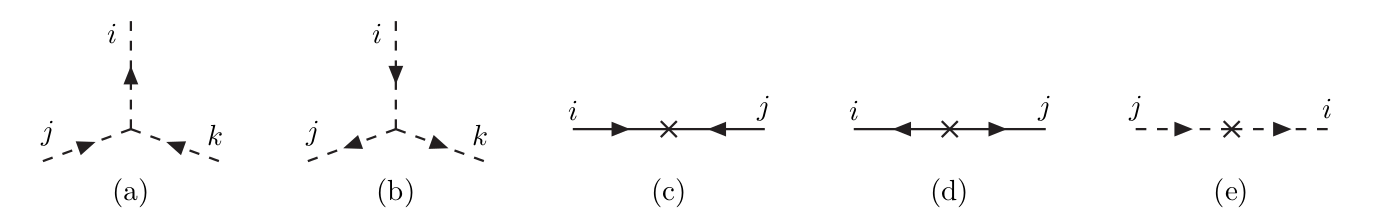
\includegraphics[scale=0.3]{images/feynman1.png}
  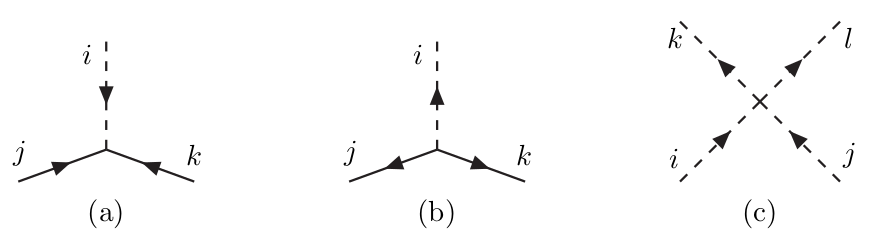
\includegraphics[scale=0.3]{images/feynman2.png}
  \caption{Interactions in the Wess-Zumino model give by the lagrangian \ref{eq:lagrangian_components}}
  \label{WZ_interactions}
\end{figure}


\newpage

\subsection*{Renormalization}

\begin{figure}[h]
  \centering
  \feynmandiagram [scale=2., layered layout, horizontal=a to c, inline=(a.base)] {
  a -- [scalar, momentum={[arrow shorten=0.3]\(p\)}] b [dot],
  b -- [scalar, momentum={[arrow shorten=0.3]\(p\)}] c,
  b -- [out=135, in=45, loop, min distance=2cm, scalar, momentum={[arrow shorten=0.3]\(q\)}] b,
}; 
\quad + \qquad
\feynmandiagram [scale=2., layered layout, horizontal=b to c, inline=(a.base)] {
  a -- [scalar, momentum={[arrow shorten=0.3]\(p\)}] b [dot],
  b -- [fermion, half left, looseness=1.5, edge label=\(q\)] c [dot],
  b -- [fermion, half right, looseness=1.5, edge label=\(p-q\)] c,
  c -- [scalar, momentum={[arrow shorten=0.3]\(p\)}] d,
};
\caption{1-loop corrections to the scalar propagator with the lagrangian give by equation ??????????????????}
\label{fig:scalar_mass_renormalization}
\end{figure}

In supersymmetry one often deals with precise cancellations of some diagrams due to the boson-fermion symmetry. As an example let us look at the scalar field's mass correction at one loop order. The two contributing diagrams are reported in figure \ref{fig:scalar_mass_renormalization}.
\raggedright The contribution from the first diagram is
\begin{gather*}
  I_1(p) = 4 \,\frac{i|y|^2}{4} \, \int \frac{d^4 q}{(2\pi)^4} \, \frac{i}{q^2 - m^2} = - |y|^2 \, \int \frac{d^4 q}{(2\pi)^4} \, \frac{1}{q^2 - m^2}
\end{gather*}
The contribution from the second diagram is 
\begin{gather*}
  I_2(p) = - 2 \, \left(\frac{iy}{2}\right)\left(\frac{iy^*}{2}\right) \int \frac{d^4 q}{(2\pi)^4} \, \text{Tr}\left[\frac{i(\sigma \cdot q + m)}{q^2 - m^2} \, \frac{i(\bar\sigma \cdot (p-q) + m)}{(p-q)^2 - m^2}\right] = \\
  - \frac{1}{2} |y|^2 \, \int \frac{d^4 q}{(2\pi)^4} \, (2) \, \frac{q\cdot p - q^2 - 2m^2}{(q^2-m^2) ((q-p)^2-m^2)}
\end{gather*}
where the property $\text{Tr}[\sigma_\mu \bar\sigma_\nu] = 2\eta_{\mu\nu}$ has been used. In order to calculate the mass renormalization, we have to evaluate the two expressions for zero incoming momentum. Hence
\begin{gather*}
  I_1(0) + I_2(0) = |y|^2 \int \frac{d^4q}{(2\pi)^4} \, \frac{1}{q^2-m^2} - \frac{q^2 -m^2 + m^2 + 2m^2}{(q^2-m^2)^2} \\
  |y|^2 \int \frac{d^4q}{(2\pi)^4} \, \cancel{\frac{1}{q^2-m^2}} - \cancel{\frac{1}{q^2-m^2}} - \frac{3m^2}{(q^2-m^2)^2}= \\ 
  = -3m^2|y|^2 \int \frac{d^4q}{(2\pi)^4} \, \frac{1}{(q^2-m^2)^2}
\end{gather*}
The quadratically divergent term got cancelled in the second line and the result is now logarithmically divergent. \\
A remarkable result which I state without proof is the so called \emph{N=1 nonrenormalization theorem}
\begin{center}
  The superpotential is never renormalised at any order in perturbation theory. Thus it might be renormalised by non-perturbative effects such as istantons.
\end{center}

\newpage 
\subsection*{Gauge theories}
We now want to introduce gauge invariance in our theory. At first let us focus on the abelian U(1) group, which will then be generalised to an arbitrary gauge group. 
Let us consider the Wess-Zumino lagrangian for an arbitrary number of superfields
\begin{equation*}
  \mathcal{L} = \int d^2\theta d^2\bar\theta \, \sum_i \Phi_i^\dagger \Phi_ii + \int d^2\theta \, \sum_i a_i \, \Phi_i + \sum_{ij} m_{ij} \, \Phi_i\Phi_j + \sum_{ijk} y_{ijk} \, \Phi_i\Phi_j\Phi_k + h.c.
\end{equation*}
Let us first consider 
a global symmetry
\begin{equation}
  \Phi \to e^{iq_i \Lambda_i}\Phi \qquad \qquad \Phi^\dagger \to \Phi^\dagger e^{-iq_i \Lambda_i}
  \label{eq:gaugetransf_phi}
\end{equation}
The kinetic term $\int d^2\theta d^2\bar\theta \sum_i \Phi_i^\dagger \Phi_i$ is always invariant but the potential term is not. In fact the linear term is obviously not invariant hence must be dropped. 
Moreover, whenever $q_i + q_j \neq 0$ we must require $m_{ij} = 0$ and whenever $q_i + q_j + q_k \neq 0$ we must require $y_{ijk} = 0$. Note in particular that diagonal terms in the mass term require $q_i + q_i = 0$ in order to be present. \\
We now promote the global symmetry to a local symmetry, hence $\Lambda \to \Lambda(x, \theta, \bar\theta)$. One can now note that the generator is not a normal function but rather a superfield. Note that it cannot be an arbitrary one. 
In fact gauge symmetries are transformations which do not change the physical state of the system, but rather configurations that differs by a gauge transformation are physically equivalent. This in particular means that a chiral field must be mapped into fields of the same chirality. 
By looking at equation \ref{eq:gaugetransfo_phi} we immediately conclude that $\Lambda(x, \theta, \bar\theta)$ must be a left-chiral superfield, hence $\Lambda^\dagger(x, \theta, \bar\theta)$ is a right-chiral superfield. \\
This immediately brings a problem in the kinetic term because 
\begin{equation*}
\Phi^\dagger \Phi \to \Phi^\dagger \, e^{-iq\Lambda^\dagger(x,\theta,\bar\theta)} \, e^{iq\Lambda(x,\theta,\bar\theta)} \, \Phi \neq \Phi^\dagger \Phi
\end{equation*}
because due to the different chirality $\Lambda^\dagger \neq \Lambda $ unless they are both constant, which is the case of global symmetry. \\
The problem is analogous to the one that one finds in the kinetic term in standard QFT when one tries to make a lagrangian gauge invariant, and it is solved by manually adding more terms. In the case of normal QFT one
promotes the derivatives to gauge covariant derivatives, here we proceed by adding a factor $e^V$ between the two superfields, where $V=V(x,\theta,\bar\theta)$ is a vector field. To see why this fixes the problem recall that a gauge transformation for any vector superfield $V$ is
\begin{equation*}
  V \to V + iq\left(\Lambda^\dagger(x, \theta, \bar\theta) - \Lambda(x, \theta, \bar\theta)\right)
\end{equation*}
which is precisely what we need. \\
Thus we must now specify a kinetic term for the gauge superfield $V(x, \theta, \bar\theta)$. This is accomplished by defining two chiral fields 
\begin{equation*}
  \mathcal{W_\alpha} \equiv -\frac{1}{4}\overline{DD}D_\alpha V \qquad \overline{\mathcal{W}}_{\dot\alpha} \equiv -\frac{1}{4}DD \overline{D}_{\dot\alpha} V
\end{equation*}
and building the two quantities
\begin{equation*}
  \mathcal{W}_{\alpha} \mathcal{W}^{\alpha} \equiv \mathcal{W}\mathcal{W} \qquad\qquad \overline{\mathcal{W}}_{\dot\alpha} \overline{\mathcal{W}}^{\dot\alpha} \equiv \overline{\mathcal{W}\mathcal{W}}
\end{equation*}
Remembering that product of superfields of the same chirality are in turn superfields of the same chirality and that the F term of a chirall field is supersymmetric invariant, the kinetic term becomes 
\begin{equation*}
  \left[\mathcal{W}\mathcal{W}\right]_F + \left[\overline{\mathcal{W}\mathcal{W}}\right]_F
\end{equation*}
The quantity is supersymmetric invariant by construction. One can make two further checks to verify that this is indeed a good choice for the kinetic term. One is gauge invariance which is straightforwardly proven using the anticommutation relation properties of the covariant derivatives $\left\{\bar{D}_{\bar\beta}, D_{\alpha}\right\}= - 2 i \sigma_{\alpha \dot{\beta}}^{\mu} \partial_{\mu}$
\begin{equation*}
  \begin{aligned}
      \mathcal{W}_{\alpha} \quad\to\quad \mathcal{W_\alpha}' &= -\frac{1}{4} \overline{D D} D_{\alpha}\left[V+i\left(\Omega^{\dagger}-\Omega\right)\right] =\mathcal{W}_{\alpha}+\frac{i}{4} \overline{D D} D_{\alpha} \Omega \\
      &=\mathcal{W}_{\alpha}-\frac{i}{4} \bar{D}^{\dot{\beta}}\left\{\bar{D}_{\dot{\beta}}, D_{\alpha}\right\} \Omega 
      =\mathcal{W}_{\alpha}+\frac{1}{2} \sigma_{\alpha \dot{\beta}}^{\mu} \partial_{\mu} \bar{D}^{\dot{\beta}} \Omega
      =\mathcal{W}_{\alpha}
  \end{aligned}
\end{equation*}
The second is to see that it at least contains the gauge spin-1 boson kinetic term. This can be done by expressing $V(x, \theta, \bar\theta)$ in compontents in the Wess-Zumino gauge and after a quite tedious but straighforward calculation one can show that 
\begin{equation*}
  \frac{1}{4} \, \left[\mathcal{W}\mathcal{W}\right]_F + \frac{1}{4} \left[\overline{\mathcal{W}\mathcal{W}}\right]_F = -\frac{1}{4} F_{\mu\nu}F^{\mu\nu} + i \lambda^\dagger \bar\sigma^\mu \partial_\mu \lambda + \frac{1}{2} \, D^2
\end{equation*}
Note that together with the usual gauge spin-1 boson kinetic term we also get a kinetic term for the spinor $\lambda$. This the fermionic superpartner of the gauge boson, the \emph{gaugino}. In the case of $U(1)$ symmetry the two superpartners are the photon and the photino.
The D term will dropout when looking at the euqation of motions. \\
In the end our abelian gauge invariant supersymmetric lagrangian is 
\begin{equation*}
  \mathcal{L} = \frac{1}{4} \, \left[\mathcal{W}\mathcal{W}\right]_F + \frac{1}{4} \left[\overline{\mathcal{W}\mathcal{W}}\right]_F + \left[\Phi^\dagger e^V \Phi\right]_D + [W(\Phi)]_F + [\overline{W} (\Phi^\dagger)]_F
\end{equation*}
The equations of motions for D are very straighforward since D is contained only in the kinetic terms through V. Noting that $[\Phi^\dagger e^V \Phi]_D = \Phi^\dagger \Phi D$ one has the equations of motions 
\begin{equation*}
  0 = \frac{d\mathcal{L}}{dD} = D + \Phi^\dagger \Phi
\end{equation*}
\par
\vspace{15pt}
The generalization to non-abelian gauge groups is conceptually straightforward, even though calculations become more complicated. Let us consider a gauge group $\mathcal{G}$ and its Lie algebra $Lie(\mathcal{G})$ with generators $\left\{T^a\right\}$.
Any element $A_\mu$ in the algebra can be written in the fundamental representation as $A_\mu = \sum_a A_\mu^a \, T^a$. The problem is that now the kinetic term in the lagrangian transforms as 
\begin{equation*}
  \Phi^\dagger e^V \Phi \to \Phi^\dagger e^{-iq\Lambda} e^{V + iq(\Lambda^\dagger - \Lambda)} e^{iq\Lambda}
\end{equation*}
which is not $\Phi^\dagger e^V \Phi$ because now the exponents have to be combined using the Baker-Campbell-Hausddorf formula. The problem can be fixed by redefining the transformation properties of the vector superfield as 
\begin{equation*}
  e^V \to e^{i\Lambda^\dagger} e^V e^{-i\Lambda}
\end{equation*}
which implies 
\begin{align*}
  V \rightarrow &V + i\left(\Omega^{\dagger}-\Omega\right)-\frac{i}{2}\left[V, \Omega+\Omega^{\dagger}\right] 
  + i \sum_{k=1}^{\infty} \frac{B_{2 k}}{(2 k) !}\left[V,\left[V, \ldots\left[V, \Omega^{\dagger}-\Omega\right] \ldots\right]\right] = \\
  = & V + i\left(\Omega^{a *}-\Omega^{a}\right)+g_{a} f^{a b c} V^{b}\left(\Omega^{c *}+\Omega^{c}\right) 
  -\frac{i}{3} g_{a}^{2} f^{a b c} f^{c d^{b}} V^{b} V^{d}\left(\Omega^{c}-\Omega^{r}\right)+\ldots
\end{align*}
where $B_n$ defined by $\frac{x}{e^{x}-1}=\sum_{n=0}^{\infty} \frac{B_{n}}{n !} x^{n}$ are the Bernoulli numbers. Note that this definition trivially reduces to the old one in the abelian case ($f^{abc}=0$). \\
The kinetic term of the gauge fields must also be redefined to take account of the new transform law of $V$ and we write it as 
\begin{equation*}
  \mathcal{W}_\alpha = -\frac{1}{4} \overline{DD} (e^{-V}D_{\alpha}e^V)
\end{equation*}
and the final lagrangian is 
\begin{equation*}
  \mathcal{L}=\frac{1}{4}\left[\mathcal{W}^{a \alpha} W_{\alpha}^{a}\right]_{F}+c . c .+\left[\Phi^{*i}\left(e^{2 g_a T^{a} V^{a}}\right)_{i}^j \Phi_{j}\right]_{D}+\left(\left[W\left(\Phi_{i}\right)\right]_F+c . c .\right) .
\end{equation*}
As an example let us write down the lagrangian in components for supersymmetric QCD and let us study it qualitatively
\begin{equation*}
  \begin{aligned}
      \mathcal{L} &=\left(D_{\mu} \varphi_{i}\right)^{*}\left(D^{\mu} \varphi\right)_{i}+\frac{i}{2} \psi_{i} \sigma^{\mu}\left(D_{\mu} \psi^{\dagger}\right)_{i}-\frac{i}{2}\left(D_{\mu} \psi\right)_{i} \sigma^{\mu} \psi^{\dagger}_{i}\\
      &-\frac{1}{4} F_{\mu \nu}^{a}\left(F^{a}\right)^{\mu \nu}+\frac{i}{2} \lambda^{a} \sigma^{\mu}\left(D_{\mu} \bar{\lambda}\right)^{a}-\frac{i}{2}\left(D_{\mu} \lambda\right)^{a} \sigma^{\mu} \bar{\lambda}^{a} \\
      &-\sqrt{2} i g \psi^{\dagger}_{i} \bar{\lambda}^{a} T_{i j}^{a} \varphi_{j}+\sqrt{2 i g} \varphi_{i}^{\dagger} T_{i j}^{a} \psi_{j} \lambda^{a} \\
      &-\frac{1}{2} \frac{\partial^{2} W}{\partial \varphi_{i} \partial \varphi_{j}} \psi_{i} \psi_{j}-\frac{1}{2} \frac{\partial^{2} W^{\dagger}}{\partial \varphi_{i}^{*} \partial \varphi_{j}^{*}} \psi^{\dagger}_{i} \psi^{\dagger}_{j}-V\left(\varphi_{i}, \varphi_{j}^{*}\right)
      \end{aligned}
\end{equation*}
where 
\begin{equation*}
    V\left(\varphi_{i}, \varphi_{j}^{*}\right)=F_{i}^{*} F_{i}+\frac{1}{2}\left(D^{a}\right)^{2}=\sum_{i}\left|\frac{\partial W}{\partial \varphi_{i}}\right|^{2}+\frac{1}{2} \sum_{a}\left(g \varphi_{i}^{*} T_{i j}^{a} \varphi_{j}+k^{a}\right)^{2}
\end{equation*}
\begin{equation*}
    W\left(\varphi_{i}\right)=a_{i} \varphi_{i}+\frac{1}{2} m_{i j} \varphi_{i} \varphi_{j}+\frac{1}{3 !} y_{i j k} \varphi_{i} \varphi_{j} \varphi_{k}
\end{equation*}
In the first line one can note the kinetic term for the quarks and the bosonic superpartners, the squarks. In the secon line there are the kinetic terms for the gluons and gluinos, in the third and fourth lines all the interactions. A peculiar and remarkable result is that the generators $T^a_{ij}$ play directly 
a role in the coupling constants. The resulting Feynman diagrams are reported below.
\begin{figure}[h]
  \centering 
  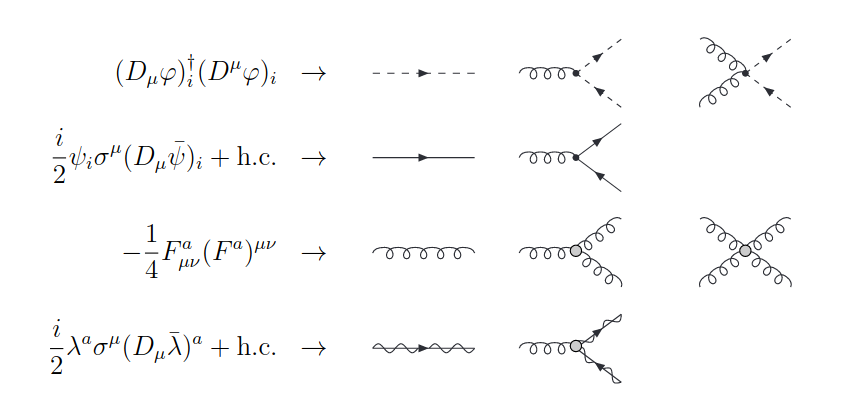
\includegraphics[scale=0.35]{sqcd_inter_2.png}
\end{figure}
\begin{figure}[h]
  \centering 
  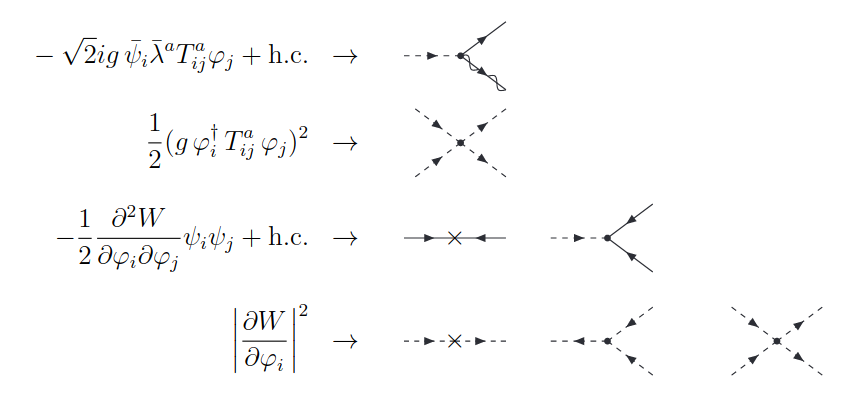
\includegraphics[scale=0.35]{sqcd_inter_1.png}
\end{figure}

\end{document}